\documentclass[11pt,notitlepage,a4paper]{article}
%\usepackage[a4paper,hmargin=1.3in,vmargin=1.3in]{geometry}
\usepackage[
  bookmarks=true,       % show bookmarks bar?
  unicode=true,         % non-Latin characters in Acrobat’s bookmarks
  pdftoolbar=false,     % show Acrobat’s toolbar?
  pdfmenubar=false,     % show Acrobat’s menu?
  pdffitwindow=false,   % window fit to page when opened
  pdfstartview={FitH},  % fits the width of the page to the window
  pdftitle={BLAKE3},    % title
  pdfauthor={TODO},     % author
  pdfsubject={BLAKE3},  % subject of the document
  pdfnewwindow=true,    % links in new window
  colorlinks=true,      % false: boxed links; true: colored links
  linkcolor=darkgreen,  % color of internal links
  citecolor=darkblue,   % color of links to bibliography
  filecolor=magenta,    % color of file links
  urlcolor=darkred,     % color of external links
]{hyperref}
\usepackage{url}
%\usepackage{fullpage}
\usepackage{a4wide}
\usepackage{amsmath,amssymb,cite,dsfont}

\usepackage{verbatim,footmisc}
\usepackage{array}

%\usepackage{euler}
%\usepackage{helvet}
%\renewcommand{\familydefault}{\sfdefault}
%\fontfamily{phv}\selectfont

\renewcommand{\familydefault}{\sfdefault}
\usepackage[scaled=1]{helvet}
\usepackage[helvet]{sfmath}
\everymath={\sf}

\usepackage[T1]{fontenc} % improves underscore rendering

\usepackage{multirow}
\usepackage{booktabs}
\usepackage{datetime}
\usepackage{xcolor}
\usepackage{graphicx}
\usepackage{subfigure}

\usepackage[english]{babel}

\usepackage{xspace}
\usepackage{booktabs}
\usepackage{listings}
\usepackage{tikz}
\usepackage[shortcuts]{extdash} % unbreakable dashes, e.g. SHA\=/2
% \usepackage[outputdir=build]{minted} % syntax highlighting using Pygments
\usepackage[title]{appendix} % add "Appendix" to each appendix section title
\usetikzlibrary
{
  calc,
  positioning,
  shapes,
  shapes.geometric,
  arrows
}

\definecolor{darkred}{RGB}{170,0,0}
\definecolor{darkblue}{RGB}{0,0,170}
\definecolor{darkgreen}{RGB}{0,170,0}

\newdateformat{mydate}{\THEYEAR.\twodigit\THEMONTH.\twodigit\THEDAY}

\newcommand{\GG}{\mathsf{G}}
\newcommand{\IV}{\text{IV}}
\newcommand{\cpress}{\text{\textbf{compress}}}
\newcommand{\lto}{\leftarrow}
\newcommand{\BB}{\mathsf{B2}}

\title{BLAKE3}

\begin{document}

\fontfamily{phv}\selectfont

\pagestyle{plain}

%\maketitle
\begin{center}
{\huge BLAKE3: one function, fast everywhere}

\bigskip

\mydate\today 
\quad---\quad
{\large \tt REQUEST FOR COMMENTS, NOT A FINAL VERSION}

\medskip

\url{https://blake3.io}

\medskip

AUTHORS
%Jack O'Connor (\texttt{@oconnor663}) \\
%Jean-Philippe Aumasson (\texttt{@veorq}) \\
%Samuel Neves (\texttt{@sevenps}) \\
%Zooko Wilcox-O'Hearn (\texttt{@zooko}) \\
%Christian Winnerlein (\texttt{@codesinchaos})
\end{center}


\medskip

\begin{center}
  \begin{minipage}{0.92\linewidth}

      \textbf{Abstract.} We present the cryptographic hash function BLAKE3, an
      improved derivative of BLAKE2 and of its predecessor, the SHA\=/3 finalist
      BLAKE. BLAKE3 supports an unbounded degree of parallelism, using an internal
      binary tree structure that scales up to any number of SIMD lanes and CPU cores.
      On Intel Kaby Lake, peak single-threaded throughput is $3\times$ that of
      BLAKE2b, $4\times$ that of SHA\=/2, and $8\times$ that of SHA\=/3, and it can scale
      further using multiple threads. On the other end, BLAKE3 is also efficient on
      smaller architectures and microcontrollers. Throughput on ARM Cortex-M0
      is $1.3\times$ that of BLAKE2s or SHA\=/256, and $3\times$ that of BLAKE2b,
      SHA\=/512, or SHA\=/3. Unlike BLAKE2 and SHA\=/2, which have incompatible
      variants better suited for different platforms, BLAKE3 is a single hash
      function, designed to be consistently fast in software across a wide
      variety of platforms and use cases.

   \end{minipage}
\end{center}

\smallskip

\section{Introduction}\label{sec:intro}

Since its announcement in 2012, BLAKE2~\cite{DBLP:conf/acns/AumassonNWW13} has 
seen widespread adoption, in large
part because of its strong performance in software. BLAKE2b and BLAKE2s are
included in OpenSSL and in the Python and Go standard libraries. BLAKE2b is
also included as the \texttt{b2sum} utility in GNU Coreutils, as the
\texttt{generichash} API in Libsodium, and as the underlying hash function for
Argon2, the winner of the Password Hashing Competition in 2015.

A drawback of BLAKE2 has been its large number of incompatible variants. The
original BLAKE2 paper described 64-bit BLAKE2b, 32-bit BLAKE2s, the parallel
variants BLAKE2bp and BLAKE2sp, and a framework for tree modes. The BLAKE2X
paper added extendable output modes. None of these are compatible with each
other, and choosing the right one for an application means understanding both
the tradeoffs between them and also the state of language and library support.
BLAKE2b, the most widely supported, is rarely the fastest on any particular
platform. BLAKE2bp and BLAKE2sp, with much higher peak throughput on x86, are
sparsely supported and almost never used.

BLAKE3 eliminates this drawback. It is a single hash function with no variants,
designed to support all the use cases of BLAKE2, as well as new use cases like
streaming verification. Furthermore, it improves on performance, in some cases
dramatically. On Intel Kaby Lake, peak throughput on a single core is triple
that of BLAKE2b, and BLAKE3 can scale further to any number of cores. On ARM
Cortex-M0, throughput is 30\% higher than BLAKE2s and again triple that of
BLAKE2b.

Internally, BLAKE3 divides its input into 2 KiB chunks and arranges those
chunks as the leaves of a binary tree. This tree structure means that there is
no limit to the parallelism that BLAKE3 can exploit, given enough input. The
direct benefit of that parallelism is very high throughput on platforms with
SIMD support, including all modern x86 processors. Another benefit of hashing
chunks in parallel is that the implementation can use SIMD vectors of any
width, regardless of the word size of the compression function. That leaves us
free to use a compression function that is efficient on smaller architectures,
without sacrificing peak throughput on x86\=/64.

The BLAKE3 compression function is closely based on BLAKE2s. BLAKE3 has the
same 128-bit security level and 256-bit default output size. The round function
is identical, along with the IV constants and the message schedule. Thus,
cryptanalysis of BLAKE2 applies directly to BLAKE3. Based on that analysis and
with the benefit of hindsight, we believe that BLAKE2 is overly conservative in
its number of rounds, and BLAKE3 reduces the number of rounds from 10 to 7.
BLAKE3 also changes the setup and finalization steps of the compression
function to support the internal tree structure, more efficient keying, and
extendable output.

The biggest changes from BLAKE2 to BLAKE3 are:

\begin{itemize}
    \item BLAKE3 uses an \textbf{internal tree structure}.
    \item There are \textbf{no variants or flavors}.
    \item The compression function uses \textbf{fewer rounds}.
    \item In lieu of a parameter block, the BLAKE3 API supports \textbf{three
        domain-separated modes}: \texttt{hash(input)},
        \texttt{keyed\_hash(key, input)}, and \texttt{derive\_key(key,
        context)}. These modes differ only in the internal flag bits they set.
    \item The space formerly occupied by the parameter block is now used for
        the optional 256-bit key, so \textbf{keying is zero-cost}.
    \item BLAKE3 has built-in support for \textbf{extendable output}. Like
        BLAKE2X, but unlike SHA\=/3 or HKDF, extended output is fully
        parallelizable.
\end{itemize}

\section{Specification}\label{sec:specification}

\subsection{Tree Structure}\label{sec:tree}

BLAKE3 splits its input into chunks of up to 2048 bytes and arranges those
chunks as the leaves of a binary tree. The last chunk may be shorter, but not
empty, unless the entire input is empty. If there is only one chunk, that chunk
is the root node and only node of the tree. Otherwise, the chunks are assembled
with parent nodes, each parent node having exactly two children. The
structure of the tree is determined by two rules:
\begin{enumerate}
    \item Left subtrees are full. Each left subtree is a complete binary tree,
        with all its chunks at the same depth, and a number of chunks that is a
        power of 2.
    \item Left subtrees are big. Each left subtree contains a number of chunks
        greater than or equal to the number of chunks in its sibling right
        subtree.
\end{enumerate}
For example, trees from 1 to 4 chunks have the structure shown in
Figure~\ref{fig:fourchunks}.

\begin{figure}[h]
\centering
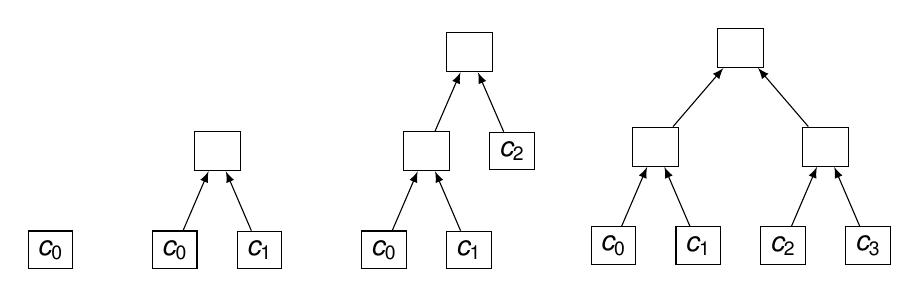
\begin{tikzpicture}

\node[draw,rectangle] (chunk1) at (0, 0) {$c_0$};

%%

\node[draw,rectangle,right=1cm of chunk1] (chunk2) {$c_0$};
\node[draw,rectangle,right=0.5cm of chunk2] (chunk3) {$c_1$};
\node[draw,rectangle,above=1cm of chunk2] (parent1) at ($(chunk2)!0.5!(chunk3)$) {\phantom{$p_0$}};
\draw[-latex] (chunk2) -- (parent1);
\draw[-latex] (chunk3) -- (parent1);

%%

\node[draw,rectangle,right=1cm of chunk3] (chunk2) {$c_0$};
\node[draw,rectangle,right=0.5cm of chunk2] (chunk3) {$c_1$};
\node[draw,rectangle,above=1cm of chunk2] (parent1) at ($(chunk2)!0.5!(chunk3)$) {\phantom{$p_0$}};
\node[draw,rectangle,right=0.5cm of parent1] (chunk4) {$c_2$};
\node[draw,rectangle,above=1cm of chunk4] (parent2) at ($(parent1)!0.5!(chunk4)$) {\phantom{$p_0$}};
\draw[-latex] (chunk2) -- (parent1);
\draw[-latex] (chunk3) -- (parent1);
\draw[-latex] (parent1) -- (parent2);
\draw[-latex] (chunk4) -- (parent2);

%%

\node[draw,rectangle,below right=1cm of chunk4] (chunk2) {$c_0$};
\node[draw,rectangle,right=0.5cm of chunk2] (chunk3) {$c_1$};
\node[draw,rectangle,above=1cm of chunk2] (parent1) at ($(chunk2)!0.5!(chunk3)$) {\phantom{$p_0$}};
\node[draw,rectangle,right=0.5cm of chunk3] (chunk4) {$c_2$};
\node[draw,rectangle,right=0.5cm of chunk4] (chunk5) {$c_3$};
\node[draw,rectangle,above=1cm of chunk4] (parent2) at ($(chunk4)!0.5!(chunk5)$) {\phantom{$p_0$}};
\node[draw,rectangle,above=1cm of parent2] (parent3) at ($(parent1)!0.5!(parent2)$) {\phantom{$p_0$}};
\draw[-latex] (chunk2) -- (parent1);
\draw[-latex] (chunk3) -- (parent1);
\draw[-latex] (chunk4) -- (parent2);
\draw[-latex] (chunk5) -- (parent2);
\draw[-latex] (parent1) -- (parent3);
\draw[-latex] (parent2) -- (parent3);

\end{tikzpicture}
\caption{Example tree structures, from 1 to 4 chunks.}
\label{fig:fourchunks}
\end{figure}

The compression function is used to derive a chaining value from each chunk and
parent node. The chaining value of the root node, encoded as 32 bytes in
little-endian order, is the default-length BLAKE3 hash of the input. BLAKE3
supports input of any byte length $0 \leq \ell < 2^{64}$.

\subsection{Compression Function}\label{sec:compression}

The compression function takes an 8-word chaining value and a 16-word message
block, and it returns a new chaining value. A word is 32 bits. The inputs to
the compression function are:

\begin{itemize}
    \item The input chaining value, $h_{0} \ldots h_{7}$.
    \item The message block, $m_{0} \ldots m_{15}$.
    \item A 64-bit offset, $t=t_{0},t_{1}$, with $t_{0}$ the lower order word
        and $t_{1}$ the higher order word.
    \item The number of input bytes in the block, $b$.
    \item A set of domain separation bit flags, $d$.
\end{itemize}

The compression function initializes its 16-word internal state $v_{0} \ldots
v_{15}$ as follows. The $\IV_{0} \ldots \IV_{7}$ constants are the same as in
BLAKE2s, and they are reproduced in appendix~\ref{sec:ivconstants}.
$\oplus$~denotes bitwise exclusive-or:

\begin{equation*}
\begin{pmatrix}
v_{0} & v_{1} & v_{2} & v_{3} \\
v_{4} & v_{5} & v_{6} & v_{7} \\
v_{8} & v_{9} & v_{10} & v_{11} \\
v_{12} & v_{13} & v_{14} & v_{15} \\
\end{pmatrix}
\leftarrow
\begin{pmatrix}
h_{0} & h_{1} & h_{2} & h_{3} \\
h_{4} & h_{5} & h_{6} & h_{7} \\
\IV_{0} & \IV_{1} & \IV_{2} & \IV_{3} \\
t_{0} \oplus \IV_{4} & t_{1} \oplus \IV_{5} & b \oplus \IV_{6} & d \oplus \IV_{7}
\end{pmatrix}
\end{equation*}

The compression function applies the round function to the state and the
message block 7 times, each time with a different message schedule. The round
function and the message schedule for each round are the same as in BLAKE2s.
They are reproduced in appendix~\ref{sec:roundfn}.

After 7 rounds of compression, the new chaining value $h_{0}' \ldots h_{7}'$ is
defined as:
\begin{align*}
    h_{0}' \ & \leftarrow \ v_{0} \oplus  v_{8} \\
    h_{1}' \ & \leftarrow \ v_{1} \oplus  v_{9} \\
    h_{2}' \ & \leftarrow \ v_{2} \oplus  v_{10} \\
    h_{3}' \ & \leftarrow \ v_{3} \oplus  v_{11} \\
    h_{4}' \ & \leftarrow \ v_{4} \oplus  v_{12} \\
    h_{5}' \ & \leftarrow \ v_{5} \oplus  v_{13} \\
    h_{6}' \ & \leftarrow \ v_{6} \oplus  v_{14} \\
    h_{7}' \ & \leftarrow \ v_{7} \oplus  v_{15}
\end{align*}

The domain separation flags used for $d$ are:
\begin{center}
\begin{tabular}{l l}
    \text{\texttt{\texttt{CHUNK}\_START}} & 1 \\
    \text{\texttt{\texttt{CHUNK\_END}}}   & 2 \\
    \text{\texttt{\texttt{PARENT}}}       & 4 \\
    \text{\texttt{\texttt{ROOT}}}         & 8 \\
    \text{\texttt{\texttt{KEYED\_HASH}}}  & 16 \\
    \text{\texttt{\texttt{DERIVE\_KEY}}}  & 32
\end{tabular}
\end{center}
The value of $d$ is the bitwise-or of all the flags set for a given
compression. Their usage is described below.

\subsection{Modes}\label{sec:modes}

BLAKE3 defines three domain-separated modes: \textbf{hash},
\textbf{keyed\_hash}, and \textbf{derive\_key}. The modes differ from each
other in their key words $k_{0} \ldots k_{7}$ and in the additional flags they
set for every call to the compression function. In the \textbf{hash} mode,
$k_{0} \ldots k_{7}$ are the constants $\IV_0 \ldots \IV_7$, and no additional
flags are set. In the \textbf{keyed\_hash} mode, $k_{0} \ldots k_{7}$ are
parsed in little-endian order from the 32-byte key given by the caller, and the
\texttt{KEYED\_HASH} flag is set for every compression. In the
\textbf{derive\_key} mode, the key is again given by the caller, and the
\texttt{DERIVE\_KEY} flag is set for every compression.

\subsection{Chunk Chaining Values}\label{sec:chunk}

Processing a chunk is structurally similar to processing input in BLAKE2s or
BLAKE2b. Each chunk of up to 2048 bytes is split into blocks of up to 64 bytes.
The last block of the last chunk may be shorter, but not empty, unless the
entire input is empty. The short block, if any, is padded with zeros to be 64
bytes. Each block is parsed in little-endian order into message words $m_{0}
\ldots m_{15}$ and compressed. The input chaining value $h_{0} \ldots h_{7}$
for the first block of each chunk is the key words $k_{0} \ldots k_{7}$. The
input chaining value for subsequent blocks in each chunk is the output of the
compression function for the previous block. The offset $t$ for each block is
the starting byte index of its chunk, 0 for all blocks in the first chunk, 2048
for all blocks in the second chunk, and so on. The block length $b$ is the
number of input bytes in each block, 64 for all blocks except the last block of
the last chunk, which may be short. The first block of each chunk sets the
\texttt{CHUNK\_START} flag, and the last block of each chunk sets the
\texttt{CHUNK\_END} flag. If a chunk contains only one block, that block sets
both \texttt{CHUNK\_START} and \texttt{CHUNK\_END}. If a chunk is the root of
its tree, the last block of that chunk also sets the \texttt{ROOT} flag. The
output of the compression function for the last block in a chunk is the
chaining value of that chunk.

\subsection{Parent Node Chaining Values}\label{sec:parent}

Each parent node has exactly two children, each either a chunk or another
parent node. The chaining value of each parent node is given by a single call
to the compression function. The input chaining value $h_{0} \ldots h_{7}$ is
the key words $k_{0} \ldots k_{7}$. The message words $m_{0} \ldots m_{15}$ are
the concatenated chaining values of the two children, first the left then the
right. The offset $t$ for parent nodes is always 0. The number of bytes $b$ for
parent nodes is always 64. Parent nodes set the \texttt{PARENT} flag. If a
parent node is the root of the tree, it also sets the \texttt{ROOT} flag. The
the output of the compression function is the chaining value of the parent
node.

\subsection{Extendable Output}\label{sec:extendable}

The default output of BLAKE3 is 32 bytes, but BLAKE3 can also produce extended
output of any byte length $\ell < 2^{64}$. This is done by repeating the root
compression --- that is, the very last call to the compression function, which
sets the \texttt{ROOT} flag --- with incrementing values of the offset $t$. The
results of these repeated root compressions are then concatenated into an
extended output.

When building an extended output, BLAKE3 uses an extended version of the
compression function that differs from the regular compression function in its
final step, returning 16 words instead of 8:
\begin{align*}
    h_{0}'  \ & \leftarrow \ v_{0} \oplus  v_{8} &
    h_{8}'  \ & \leftarrow \ v_{8} \oplus  h_{0} \\
    h_{1}'  \ & \leftarrow \ v_{1} \oplus  v_{9} &
    h_{9}'  \ & \leftarrow \ v_{9} \oplus  h_{1} \\
    h_{2}'  \ & \leftarrow \ v_{2} \oplus  v_{10} &
    h_{10}' \ & \leftarrow \ v_{10} \oplus  h_{2} \\
    h_{3}'  \ & \leftarrow \ v_{3} \oplus  v_{11} &
    h_{11}' \ & \leftarrow \ v_{11} \oplus  h_{3} \\
    h_{4}'  \ & \leftarrow \ v_{4} \oplus  v_{12} &
    h_{12}' \ & \leftarrow \ v_{12} \oplus  h_{4} \\
    h_{5}'  \ & \leftarrow \ v_{5} \oplus  v_{13} &
    h_{13}' \ & \leftarrow \ v_{13} \oplus  h_{5} \\
    h_{6}'  \ & \leftarrow \ v_{6} \oplus  v_{14} &
    h_{14}' \ & \leftarrow \ v_{14} \oplus  h_{6} \\
    h_{7}'  \ & \leftarrow \ v_{7} \oplus  v_{15} &
    h_{15}' \ & \leftarrow \ v_{15} \oplus  h_{7}
\end{align*}
Note that the first 8 words of the extended compression output are the same as
the regular compression output. The last 8 words are the input chaining value
fed forward into the last 8 words of the internal state. Each 16-word output is
encoded as 64 bytes in little-endian order.

Observe that for the default output, the root compression always uses offset $t
= 0$. That is either because it is the last block of the only chunk, which has
a chunk offset of $0$, or because it is a parent node. For extended output, the
first root compression sets $t = 0$ as usual but uses the extended compression
function. Then as long as more bytes are needed, $t$ is incremented by 64, and
the root compression is repeated on the same inputs. If the target output
length is not a multiple of 64, the final compression output is truncated.

Because the repeated root compressions differ only in the value of $t$, the
implementation can execute any number of them in parallel. The caller can also
adjust $t$ to seek to any point in the output stream.

Note that in contrast to BLAKE2 and BLAKE2X, BLAKE3 does not domain separate
outputs of different lengths. Shorter outputs are prefixes of longer ones.

\section{Performance}\label{sec:performance}

It's fast :)

\section{Security}\label{sec:security}

It's safe :)

\section{Memory Requirement}\label{sec:memory}

It's big :(

\section{Implementation}\label{sec:implementation}

\subsection{SIMD}\label{sec:simd}

There are two approaches to using SIMD in a BLAKE3 implementation, and both are
important for high performance at different input lengths. The first approach
is to use 128-bit vectors to represent the 4-word rows of the state matrix. The
second approach is to use vectors of any size to represent words in multiple
states, which are compressed in parallel.

The first approach is similar to how SIMD is used in BLAKE2b or BLAKE2s, and it
is applicable to inputs of any length, particularly short inputs where the
second approach does not apply. The state $v_0 \ldots v_{15}$ is arranged into
four 128-bit vectors. The first vector contains the state words $v_0 \ldots
v_3$, the second vector contains the state words $v_4 \ldots v_7$, and so on.
Implementing the G function (Appendix~\ref{sec:roundfn}) with vector
instructions thus mixes all four columns of the state matrix in parallel. A
diagonalization step then rotates the words within each row so that each
diagonal now lies along a column, and the vectorized G function is repeated to
mix diagonals. Finally the state is undiagonalized, to prepare for the column
step of the following round.

The second approach is similar to how SIMD is used in BLAKE2bp or BLAKE2sp. In
this approach, multiple chunks are compressed in parallel, and each vector
contains one word from the state matrix of each chunk. That is, the first
vector contains the $v_0$ word from each state, the second vector contains the
$v_1$ word from each state, and so on, using 16 vectors in total. The width of
the vectors determines the number of chunks, so for example 128-bit vectors
compress 4 chunks in parallel, and 256-bit vectors compress 8 chunks in
parallel. Here the G function operates on one column or diagonal at a time, but
across all of the states, and no diagonalization step is required. When enough
input is available, this approach is much more efficient than the first
approach. It also scales to wider instruction sets like AVX2 and AVX-512.

\subsection{Incremental Hashing}\label{sec:incremental}

How to merge subtrees, using that trick with counting 1 bits. Include a pretty
diagram.

\section{Applications}\label{sec:applications}

\subsection{Message Authentication Codes}\label{sec:mac}

Like BLAKE2, BLAKE3 has explicit support for a keyed mode,
\textbf{keyed\_hash}. This removes the need for a separate construction like
HMAC. The \textbf{keyed\_hash} mode is also more efficient than keyed BLAKE2 or
HMAC for short messages. BLAKE2 requires an extra compression for the key
block, and HMAC requires three extra compressions. The \textbf{keyed\_hash}
mode in BLAKE3 does not require any extra compressions.

\subsection{Key Derivation}\label{sec:kdf}

BLAKE3 has explicit support for a key derivation mode, \textbf{derive\_key}.
The input bytes should be a hardcoded, globally unique context string. A good
default format for such strings is \texttt{"[application] [date] [purpose]"}, e.g.,
\texttt{"example.com 2019-12-25 16:18:03 session tokens v1"}. If the input key material
is not already a 256-bit key, it should first be converted into 256 bits using
the default output of the BLAKE3 \textbf{hash} mode.

The \textbf{derive\_key} mode is intended to replace the BLAKE2 personalization
parameter for its most common use cases. Like \textbf{keyed\_hash}, it does not
require any extra compressions. For context strings up to 64 bytes and derived
key lengths up to 64 bytes, \textbf{derive\_key} is a single compression.

Key derivation can encourage better security than personalization, by
cryptographically isolating different components of an application from one
another. This limits the damage that one component can cause by accidentally
leaking its key. When an application needs to use one secret in multiple
algorithms or contexts, the best practice is to derive a separate key for each
use case, such that the original secret is only used with the key derivation
function. However, because the BLAKE3 modes are domain-separated, it is also
possible to use the same key with \textbf{keyed\_hash} and with
\textbf{derive\_key}. This can be necessary for backwards compatibility when an
application adds a new use case for an existing key, if the original use case
did not include a context-specific key derivation step.

\subsection{Streaming Verification}\label{sec:streamingverification}

Bao, basically.

\subsection{Incremental Update}\label{sec:incrementalupdate}

Giant disk images.

\section{Rationales}\label{sec:rationales}

\nocite{*}
\bibliographystyle{plainurl}
\bibliography{blake3}

[These references are placeholders. TODO.]

\begin{appendices}

\section{IV Constants}\label{sec:ivconstants}

    The constants $\IV_0 \ldots \IV_7$ used by the compression function are the
    same as in BLAKE2s. They are:
\begin{align*}
    \IV_0 &= \text{\texttt{0x6a09e667}} &
    \IV_1 &= \text{\texttt{0xbb67ae85}} \\
    \IV_2 &= \text{\texttt{0x3c6ef372}} &
    \IV_3 &= \text{\texttt{0xa54ff53a}} \\
    \IV_4 &= \text{\texttt{0x510e527f}} &
    \IV_5 &= \text{\texttt{0x9b05688c}} \\
    \IV_6 &= \text{\texttt{0x1f83d9ab}} &
    \IV_7 &= \text{\texttt{0x5be0cd19}}
\end{align*}

\section{Round Function}\label{sec:roundfn}

    The compression function transforms the internal state $v_{0} \ldots
    v_{15}$ through a sequence of 7 rounds. The round function is the same as
    in BLAKE2s. A round does:
\begin{align*}
    \GG_{0}&(v_{0}, v_{4}, v_{8}, v_{12}) &
    \GG_{1}&(v_{1}, v_{5}, v_{9}, v_{13}) &
    \GG_{2}&(v_{2}, v_{6}, v_{10}, v_{14}) &
    \GG_{3}&(v_{3}, v_{7}, v_{11}, v_{15}) \\
    \GG_{4}&(v_{0}, v_{5}, v_{10}, v_{15}) &
    \GG_{5}&(v_{1}, v_{6}, v_{11}, v_{12}) &
    \GG_{6}&(v_{2}, v_{7}, v_{8}, v_{13}) &
    \GG_{7}&(v_{3}, v_{4}, v_{9}, v_{14})
\end{align*}

    That is, a round applies a G function to each of the columns in parallel,
    and then to each of the diagonals in parallel. $\GG_i(a, b, c, d)$ is
    defined as follows. $\ggg$~denotes bitwise right rotation, and
    $m_{\sigma_r(x)}$ is the message word whose index is the
    $x$\textsuperscript{th} entry in the message schedule for round $r$:
\begin{align*}
    a \ & \leftarrow \ a + b + m_{\sigma_r(2i)} \\
    d \ & \leftarrow \ (d \oplus a) \ggg 16 \\
    c \ & \leftarrow \ c + d \\
    b \ & \leftarrow \ (b \oplus c) \ggg 12 \\
    a \ & \leftarrow \ a + b + m_{\sigma_r(2i+1)} \\
    d \ & \leftarrow \ (d \oplus a) \ggg 8 \\
    c \ & \leftarrow \ c + d \\
    b \ & \leftarrow \ (b \oplus c) \ggg 7
\end{align*}

    The message schedules $\sigma_r$ are:

\begin{center}
\begin{tabular}{ | r | r r r r r r r r r r r r r r r r | }
    \hline
    $\sigma_0$ & 0 & 1 & 2 & 3 & 4 & 5 & 6 & 7 & 8 & 9 & 10 & 11 & 12 & 13 & 14 & 15 \\
    $\sigma_1$ & 14 & 10 & 4 & 8 & 9 & 15 & 13 & 6 & 1 & 12 & 0 & 2 & 11 & 7 & 5 & 3 \\
    $\sigma_2$ & 11 & 8 & 12 & 0 & 5 & 2 & 15 & 13 & 10 & 14 & 3 & 6 & 7 & 1 & 9 & 4 \\
    $\sigma_3$ & 7 & 9 & 3 & 1 & 13 & 12 & 11 & 14 & 2 & 6 & 5 & 10 & 4 & 0 & 15 & 8 \\
    $\sigma_4$ & 9 & 0 & 5 & 7 & 2 & 4 & 10 & 15 & 14 & 1 & 11 & 12 & 6 & 8 & 3 & 13 \\
    $\sigma_5$ & 2 & 12 & 6 & 10 & 0 & 11 & 8 & 3 & 4 & 13 & 7 & 5 & 15 & 14 & 1 & 9 \\
    $\sigma_6$ & 12 & 5 & 1 & 15 & 14 & 13 & 4 & 10 & 0 & 7 & 6 & 3 & 9 & 2 & 8 & 11 \\
    \hline
\end{tabular}
\end{center}

% \section{Rust Reference Implementation}\label{sec:referenceimpl}

% \inputminted[fontsize=\footnotesize]{rust}{reference_impl.rs}

\end{appendices}

\end{document}
